\section{Technique and implementation}
%% \label{sec:approach}

\begin{figure*}
  \centering
  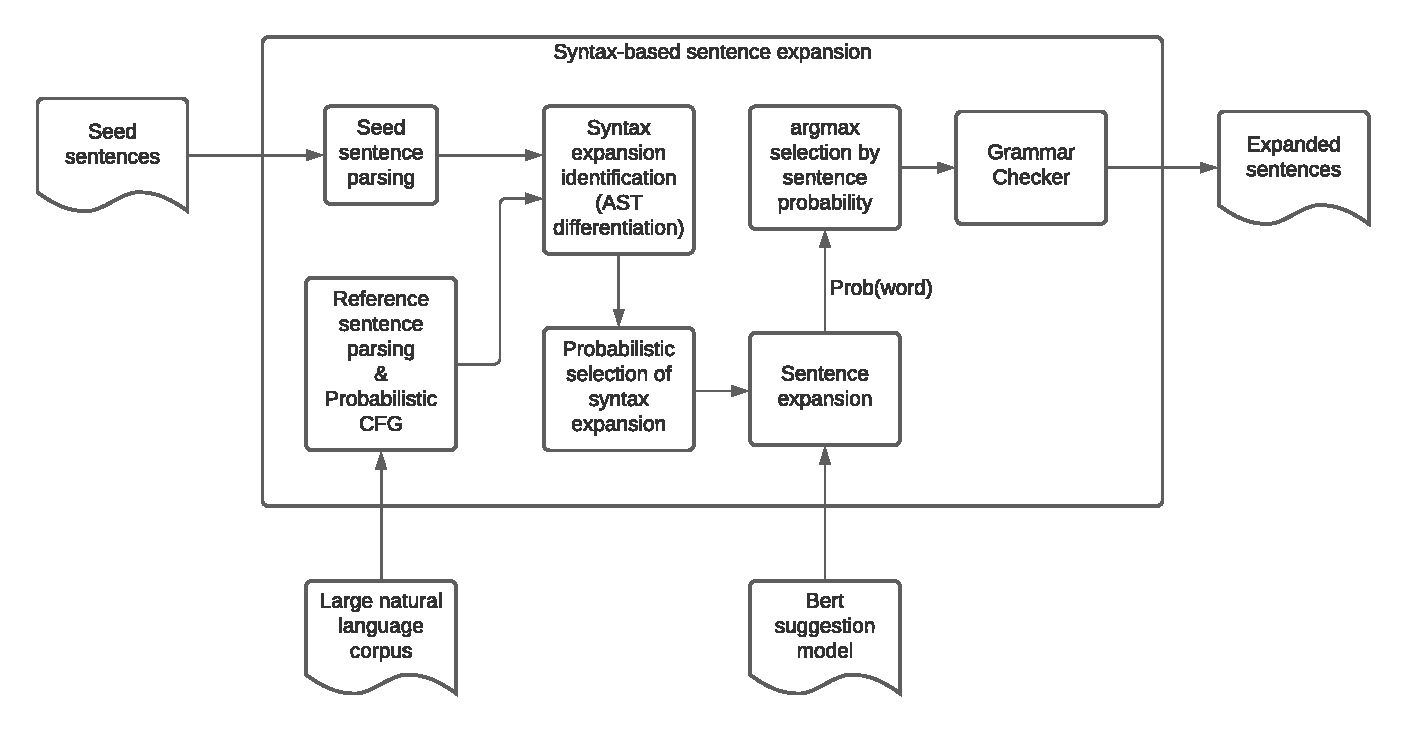
\includegraphics[scale=0.5]{figs/overall.pdf}
  \vspace{-5pt}
  \caption{\OverallModelFigCaption}
  \vspace{-10pt}
\end{figure*}

\Model generates input sentences with the following phases illustrated
in \ref{fig:OverallModel}: 1. search phase searches seed sentences according to
its requirement of \lc, 2. seed parsing phase parses the found seed
sentences and extract their \cfg, 3. reference phase collects large
corpus, 4. syntax expansion identification, and 5.sentence expansion
and generation. In this section, we provide more details on each phase.

\subsection{Search phase}
The search phase in \Model searches inputs in dataset and selects
subset of input sentences in the dataset that meets the \lc
requirement. The idea behind this phase is that input distribution of
\lc is important to generate inputs relevant to \lc. \Lc describes
expected behaviors of NLP model on specific types of input and
output. The NLP model is evaluated on how much it performs on the
input and output. Thus, \lc introduces the constraints of the input
data. Input data from the constrained distribution are only qualified
to be used for evaluating the NLP model on the \lc.  In addition,
diversity in inputs is important to evaluate NLP models on the
\lc. Inputs that differ are more likely to cover the NLP model
behavior, and more coverage increases trustworthiness of the
evaluation. To satisfy the same distribution and high
diversity among inputs, we estabilish requirement of input and output
for each \lc, and find inputs that fulfil the requirements.
